\newpage
\lecture{15}{Теорема Радона-Никодима. Теорема Фубини.}

\subsection{Знакопеременные меры.}

\begin{definition}
    Пусть $(X,\, \CE)$~--- измеримое пространство.
    Пусть $\mu:\: \CE\to\R$ такая, что $\mu(\varnothing)=0$ и \[
        \mu\left(\bigsqcup_{k=1}^{\infty}A_k\right)
        =\sum_{k=1}^{\infty}\mu(A_k),\quad\forall
        \{A_k\}_{k=1}^{\infty}\subset\CE.
    \]
    Тогда $\mu$ называется \mdef{знакопеременной мерой.}

    \begin{remark}
        Пусть $\mu$~--- знакопеременная мера, $E\in\CE$.
        Тогда функция $\mu|_E:\:\CE\to\R$ (или $\CE\to[0,\, +\infty]$, в случае неотрицательной меры)
        такая, что $\mu|_E(A):=\mu(A\cap E)$, называется \mdef{ограничением} (\mdef{сужением})
        $\mu$ на множество $E$.
    \end{remark}
\end{definition}

\begin{theorem}[Хана-Жордана]
    Пусть $\mu$~--- знакопеременная мера.
    Тогда существует множество $X^+\in\CE:\: \mu_{X^+}\geqslant 0$
    и $\mu_{X^-}\leqslant 0$, где $X^-=X\setminus X^+$.

    \begin{proof}

        Рассмотрим \[
            \CE_{-}=\{E\in\CE:\: \mu|_E\leqslant0\},
        \]
        где $\mu|_E\leqslant 0$ означает, что $\forall B\in\CE:\: \mu|_E(B)\leqslant 0$.

        Пусть \[
            \beta:=\inf \{\mu(E):\: E\in\CE_-\}.
        \]
        Заметим, что инфинум достигается, то есть $\exists E\in\CE_-:\: \beta=\mu(E)$.
        Действительно, рассмотрим последовательность $\{E_n\}_{n\in\N},\, E_n\in\CE$ такую,
        что $\mu(E_n)\xrightarrow[n\toi]{}\beta$. Тогда
        пусть \[
            E:=\bigcup\limits_{k=1}^{\infty}E_k=\bigsqcup\limits_{k=1}^{\infty}E_k',
            \quad \text{где } E_k'=E_k\setminus \bigcup_{j=1}^{k-1}E_j\in\CE_-.
        \]
        Тогда \[
            \mu(E)=\sum_{k=1}^{\infty}\mu(E_k')=\lim_{n\toi}\sum_{k=1}^{n}\mu(E_k')=
            \lim_{n\toi}\mu\left(\bigsqcup_{k=1}^{n}E_k'\right)=
            \lim_{n\toi}\mu(E_n)=\beta.
        \]
        Далее, $\mu|_E\leqslant 0$, так как \[
            \mu|_E(A)=\mu(E\cap A)=\sum_{k=1}^{\infty}\underbrace{\mu(E_k'\cap A)}_{\leqslant 0}\leqslant0.
        \]

        Возьмем, $X^-:=E,\, X^+=X\setminus E$.
        Докажем, что $\mu|_{X^+}\geqslant 0$. Предположим, что это не так.
        То есть $\exists B\subset X^+$ такое, что $\mu(B)<0$.
        Заметим, что $\forall n\in\N$ существует не более чем конечное дизъюнктное
        семейство множеств $\{B_k\}:\: \mu(B_k)>\dfrac{1}{n}$ (см. рис. ниже), в самом деле,
        иначе получим, что \[
            \mu\left(\bigsqcup_{k=1}^{\infty}B_k\right)=\sum_{k=1}^{\infty}\mu(B_k)=+\infty.
        \]

        \begin{center}
            

% Pattern Info
 
\tikzset{
pattern size/.store in=\mcSize, 
pattern size = 5pt,
pattern thickness/.store in=\mcThickness, 
pattern thickness = 0.3pt,
pattern radius/.store in=\mcRadius, 
pattern radius = 1pt}
\makeatletter
\pgfutil@ifundefined{pgf@pattern@name@_m5ideafz4}{
\pgfdeclarepatternformonly[\mcThickness,\mcSize]{_m5ideafz4}
{\pgfqpoint{0pt}{0pt}}
{\pgfpoint{\mcSize+\mcThickness}{\mcSize+\mcThickness}}
{\pgfpoint{\mcSize}{\mcSize}}
{
\pgfsetcolor{\tikz@pattern@color}
\pgfsetlinewidth{\mcThickness}
\pgfpathmoveto{\pgfqpoint{0pt}{0pt}}
\pgfpathlineto{\pgfpoint{\mcSize+\mcThickness}{\mcSize+\mcThickness}}
\pgfusepath{stroke}
}}
\makeatother
\tikzset{every picture/.style={line width=0.75pt}} %set default line width to 0.75pt        

\begin{tikzpicture}[x=0.75pt,y=0.75pt,yscale=-1,xscale=1]
%uncomment if require: \path (0,300); %set diagram left start at 0, and has height of 300

%Shape: Ellipse [id:dp25988630439456917] 
\draw  [fill={rgb, 255:red, 255; green, 255; blue, 255 }  ,fill opacity=1 ] (30,145) .. controls (30,70.44) and (115.07,10) .. (220,10) .. controls (324.93,10) and (410,70.44) .. (410,145) .. controls (410,219.56) and (324.93,280) .. (220,280) .. controls (115.07,280) and (30,219.56) .. (30,145) -- cycle ;
%Curve Lines [id:da46349619352922966] 
\draw    (161.8,16.75) .. controls (211.3,54.05) and (119.3,215.95) .. (157.8,272.95) ;
%Shape: Polygon Curved [id:ds587797750584931] 
\draw  [color={rgb, 255:red, 208; green, 2; blue, 27 }  ,draw opacity=1 ][pattern=_m5ideafz4,pattern size=16.5pt,pattern thickness=0.75pt,pattern radius=0pt, pattern color={rgb, 255:red, 126; green, 211; blue, 33}] (203.8,49.75) .. controls (221.8,16.25) and (285.8,2.25) .. (336.3,90.75) .. controls (386.8,179.25) and (366.8,197.75) .. (362.3,204.25) .. controls (357.8,210.75) and (226.3,278.25) .. (206.3,248.25) .. controls (186.3,218.25) and (185.8,83.25) .. (203.8,49.75) -- cycle ;
%Shape: Circle [id:dp3591769407303209] 
\draw  [color={rgb, 255:red, 189; green, 16; blue, 224 }  ,draw opacity=1 ][fill={rgb, 255:red, 255; green, 255; blue, 255 }  ,fill opacity=1 ] (203.25,86.63) .. controls (203.25,79.24) and (209.24,73.25) .. (216.63,73.25) .. controls (224.01,73.25) and (230,79.24) .. (230,86.63) .. controls (230,94.01) and (224.01,100) .. (216.63,100) .. controls (209.24,100) and (203.25,94.01) .. (203.25,86.63) -- cycle ;
%Shape: Circle [id:dp41983172793902224] 
\draw  [color={rgb, 255:red, 189; green, 16; blue, 224 }  ,draw opacity=1 ][fill={rgb, 255:red, 255; green, 255; blue, 255 }  ,fill opacity=1 ] (203.25,123.38) .. controls (203.25,115.99) and (209.24,110) .. (216.63,110) .. controls (224.01,110) and (230,115.99) .. (230,123.38) .. controls (230,130.76) and (224.01,136.75) .. (216.63,136.75) .. controls (209.24,136.75) and (203.25,130.76) .. (203.25,123.38) -- cycle ;
%Shape: Circle [id:dp4206296595453043] 
\draw  [color={rgb, 255:red, 189; green, 16; blue, 224 }  ,draw opacity=1 ][fill={rgb, 255:red, 255; green, 255; blue, 255 }  ,fill opacity=1 ] (203.25,156.63) .. controls (203.25,149.24) and (209.24,143.25) .. (216.63,143.25) .. controls (224.01,143.25) and (230,149.24) .. (230,156.63) .. controls (230,164.01) and (224.01,170) .. (216.63,170) .. controls (209.24,170) and (203.25,164.01) .. (203.25,156.63) -- cycle ;
%Shape: Circle [id:dp0216623369416995] 
\draw  [color={rgb, 255:red, 245; green, 166; blue, 35 }  ,draw opacity=1 ][fill={rgb, 255:red, 255; green, 255; blue, 255 }  ,fill opacity=1 ] (250,61.5) .. controls (250,56.81) and (253.81,53) .. (258.5,53) .. controls (263.19,53) and (267,56.81) .. (267,61.5) .. controls (267,66.19) and (263.19,70) .. (258.5,70) .. controls (253.81,70) and (250,66.19) .. (250,61.5) -- cycle ;
%Shape: Circle [id:dp9650486647778433] 
\draw  [color={rgb, 255:red, 245; green, 166; blue, 35 }  ,draw opacity=1 ][fill={rgb, 255:red, 255; green, 255; blue, 255 }  ,fill opacity=1 ] (250,88.5) .. controls (250,83.81) and (253.81,80) .. (258.5,80) .. controls (263.19,80) and (267,83.81) .. (267,88.5) .. controls (267,93.19) and (263.19,97) .. (258.5,97) .. controls (253.81,97) and (250,93.19) .. (250,88.5) -- cycle ;
%Shape: Circle [id:dp33413294409784267] 
\draw  [color={rgb, 255:red, 245; green, 166; blue, 35 }  ,draw opacity=1 ][fill={rgb, 255:red, 255; green, 255; blue, 255 }  ,fill opacity=1 ] (250,111.5) .. controls (250,106.81) and (253.81,103) .. (258.5,103) .. controls (263.19,103) and (267,106.81) .. (267,111.5) .. controls (267,116.19) and (263.19,120) .. (258.5,120) .. controls (253.81,120) and (250,116.19) .. (250,111.5) -- cycle ;
%Shape: Circle [id:dp8843033103309779] 
\draw  [color={rgb, 255:red, 245; green, 166; blue, 35 }  ,draw opacity=1 ][fill={rgb, 255:red, 255; green, 255; blue, 255 }  ,fill opacity=1 ] (250,138.5) .. controls (250,133.81) and (253.81,130) .. (258.5,130) .. controls (263.19,130) and (267,133.81) .. (267,138.5) .. controls (267,143.19) and (263.19,147) .. (258.5,147) .. controls (253.81,147) and (250,143.19) .. (250,138.5) -- cycle ;
%Shape: Circle [id:dp5263060284536751] 
\draw  [color={rgb, 255:red, 74; green, 144; blue, 226 }  ,draw opacity=1 ][fill={rgb, 255:red, 255; green, 255; blue, 255 }  ,fill opacity=1 ] (240,223) .. controls (240,219.13) and (243.13,216) .. (247,216) .. controls (250.87,216) and (254,219.13) .. (254,223) .. controls (254,226.87) and (250.87,230) .. (247,230) .. controls (243.13,230) and (240,226.87) .. (240,223) -- cycle ;
%Shape: Circle [id:dp4015620631666985] 
\draw  [color={rgb, 255:red, 74; green, 144; blue, 226 }  ,draw opacity=1 ][fill={rgb, 255:red, 255; green, 255; blue, 255 }  ,fill opacity=1 ] (256,203) .. controls (256,199.13) and (259.13,196) .. (263,196) .. controls (266.87,196) and (270,199.13) .. (270,203) .. controls (270,206.87) and (266.87,210) .. (263,210) .. controls (259.13,210) and (256,206.87) .. (256,203) -- cycle ;
%Shape: Circle [id:dp8219755725352689] 
\draw  [color={rgb, 255:red, 74; green, 144; blue, 226 }  ,draw opacity=1 ][fill={rgb, 255:red, 255; green, 255; blue, 255 }  ,fill opacity=1 ] (280,213) .. controls (280,209.13) and (283.13,206) .. (287,206) .. controls (290.87,206) and (294,209.13) .. (294,213) .. controls (294,216.87) and (290.87,220) .. (287,220) .. controls (283.13,220) and (280,216.87) .. (280,213) -- cycle ;
%Shape: Circle [id:dp8336297949289684] 
\draw  [color={rgb, 255:red, 74; green, 144; blue, 226 }  ,draw opacity=1 ][fill={rgb, 255:red, 255; green, 255; blue, 255 }  ,fill opacity=1 ] (286,187) .. controls (286,183.13) and (289.13,180) .. (293,180) .. controls (296.87,180) and (300,183.13) .. (300,187) .. controls (300,190.87) and (296.87,194) .. (293,194) .. controls (289.13,194) and (286,190.87) .. (286,187) -- cycle ;

% Text Node
\draw (390,215.5) node [anchor=north west][inner sep=0.75pt]  [font=\LARGE] [align=left] {$\displaystyle X$};
% Text Node
\draw (52,139.5) node [anchor=north west][inner sep=0.75pt]  [font=\LARGE] [align=left] {$\displaystyle E$};
% Text Node
\draw (221,40) node [anchor=north west][inner sep=0.75pt]   [align=left] {$\displaystyle \textcolor[rgb]{0.82,0.01,0.11}{B}$};
% Text Node
\draw (197,180) node [anchor=north west][inner sep=0.75pt]  [color={rgb, 255:red, 189; green, 16; blue, 224 }  ,opacity=1 ] [align=left] {$\displaystyle \mu  >1$};
% Text Node
\draw (271,72) node [anchor=north west][inner sep=0.75pt]  [color={rgb, 255:red, 245; green, 166; blue, 35 }  ,opacity=1 ] [align=left] {$\displaystyle \mu  >\frac{1}{2}$};
% Text Node
\draw (311,160) node [anchor=north west][inner sep=0.75pt]  [color={rgb, 255:red, 74; green, 144; blue, 226 }  ,opacity=1 ] [align=left] {$\displaystyle \mu  >\frac{1}{3}$};
% Text Node
\draw (288,125.5) node [anchor=north west][inner sep=0.75pt]  [font=\LARGE] [align=left] {$\displaystyle \textcolor[rgb]{0.49,0.83,0.13}{D}$};


\end{tikzpicture}

        \end{center}

        Обобщая можем написать, что существует не более чем счетное дизъюнктное семейство
        $\{P_k\}_{k=1}^{\infty}\subset B$ такое, что $\mu(P_k)>0$ и
        не существует множества
        $A\subset B\setminus \bigsqcup\limits_{k=1}^{\infty}P_k=:D:\: \mu(A)>0$.

        Но тогда просто по определению, $\mu|_{D}\leqslant 0$.
        Итак, \[
            \mu(D)=\mu(B)-\mu\left(\bigsqcup_{k=1}^{\infty}P_k\right)
            =\mu(B)-\sum_{k=1}^{\infty}\underbrace{\mu(P_k)}_{>0}<\mu(B)<0.
        \]
        Но тогда получается, что $\mu|_D\leqslant 0\Rightarrow \mu|_{E\cup D}\leqslant 0$
        и $\mu(E\sqcup D)=\mu(E)+\mu(D)<\mu(E)=\beta$~--- противоречие (несостыковка
        с инфинумом).

    \end{proof}
\end{theorem}

\begin{definition}
    Пусть $\mu,\, \nu:\: \CE\to[0,\, +\infty]$~--- $\sigma$"=аддитивные меры, где
    $(X,\, \CE)$~--- измеримое пространство.

    Будем говорить, что $\nu\ll\mu$ (\mdef{абсолютно непрерывна} относительно
    $\mu$), если \[
        \forall N\in\CE\quad \mu(N)=0\Rightarrow \nu(N)=0.
    \]

    Будем говорить, что $\nu\bot \mu$ ($\nu$ и $\mu$\mdef{взаимно сингулярны}),
    если $\exists E\in\CE$ такое, что $\nu$ сосредоточена на $E$, а
    $\mu$ сосредоточена на $E^C$.

    Мера $\nu$\mdef{сосредоточена} на $E$ означает, что $\forall F\subset E^C\ (F\in\CE):\:
        \nu(F)=0$.

    \begin{remark}
        Данные определения имеют смысл также и для знакопеременных мер.
    \end{remark}
\end{definition}

\begin{exercise}
    Пусть \[
        \delta_x(A)=\begin{cases}
            1, & x\in A,    \\
            0, & x\notin A.
        \end{cases}\text{~---\mdef{мера Дирака, сосредоточенная в точке $x$}.}
    \]

    Рассмотрим $X=\R$ и $\CE=2^{\R}$. Тогда
    \begin{align*}
         & \delta_0\ll\delta_0+\delta_1, \\
         & \delta_0\bot\delta_1,
    \end{align*}
    где $(\mu+\nu)(A)=\mu(A)+\nu(A)$.
\end{exercise}

\begin{exercise}
    Пусть $\lambda$~--- мера Лебега на $\R$, $f\in L^1(\R)$ и \[
        \nu(A):=\int_A fd\lambda\Rightarrow \nu\ll\lambda.
    \]
\end{exercise}

\begin{definition}
    Данная в примере выше $f$ называется\mdef{плотностью} $\nu$ относительно $\mu$.

    Также используют термин\mdef{производная Радона-Никодима}.

    Обозначение: $f=\dfrac{d\nu}{d\mu}$.
\end{definition}

\begin{theorem}[Радон-Никодим]
    Пусть $\nu,\, \mu:\:\CE\to[0,\, +\infty]$~--- $\sigma$"=конечные,
    $\sigma$"=аддитивные на $(X,\, \CE)$ меры.

    Если $\nu\ll\mu$, то существует $f:\: X\to[0,\, +\infty)$
    измеримая относительно $\CE$ такая, что
    \[
        \forall A\in\CE:\quad \nu(A)=\int_A fd\mu.
    \]

    \begin{proof}

        \underline{\textit{Общая идея.}}
        Пусть такая $f$ существует. Для примера рассмотрим случай, когда в качестве
        $\mu$ берется мера Лебега.
        Нарисуем график функции $f$. Нужно найти $f$ не зная ее заранее.
        Для этого будем проводить горизонтальные прямые (на высоте $\varepsilon$).
        Тогда $X$ разбивается на две части, где функция больше чем $\varepsilon$ и
        где меньше. Возникает вопрос, какая мера у множества, на котором $f\geqslant\varepsilon$?

        Итак, $\forall\varepsilon>0$ рассмотрим $\{f\geqslant \varepsilon\}\sqcup
            \{f<\varepsilon\}=X$ (см. рис. ниже).

        \begin{center}
            

% Pattern Info
 
\tikzset{
pattern size/.store in=\mcSize, 
pattern size = 5pt,
pattern thickness/.store in=\mcThickness, 
pattern thickness = 0.3pt,
pattern radius/.store in=\mcRadius, 
pattern radius = 1pt}
\makeatletter
\pgfutil@ifundefined{pgf@pattern@name@_fyojed01u}{
\pgfdeclarepatternformonly[\mcThickness,\mcSize]{_fyojed01u}
{\pgfqpoint{0pt}{0pt}}
{\pgfpoint{\mcSize+\mcThickness}{\mcSize+\mcThickness}}
{\pgfpoint{\mcSize}{\mcSize}}
{
\pgfsetcolor{\tikz@pattern@color}
\pgfsetlinewidth{\mcThickness}
\pgfpathmoveto{\pgfqpoint{0pt}{0pt}}
\pgfpathlineto{\pgfpoint{\mcSize+\mcThickness}{\mcSize+\mcThickness}}
\pgfusepath{stroke}
}}
\makeatother
\tikzset{every picture/.style={line width=0.75pt}} %set default line width to 0.75pt        

\begin{tikzpicture}[x=0.75pt,y=0.75pt,yscale=-1,xscale=1]
%uncomment if require: \path (0,300); %set diagram left start at 0, and has height of 300

%Curve Lines [id:da2009657115584773] 
\draw    (40,230) .. controls (99.7,230.25) and (120.8,160.25) .. (160,160) .. controls (199.2,159.75) and (220.7,229.25) .. (280,230) ;
%Straight Lines [id:da08665955983676965] 
\draw    (30,240) -- (298,240) ;
\draw [shift={(300,240)}, rotate = 180] [color={rgb, 255:red, 0; green, 0; blue, 0 }  ][line width=0.75]    (10.93,-3.29) .. controls (6.95,-1.4) and (3.31,-0.3) .. (0,0) .. controls (3.31,0.3) and (6.95,1.4) .. (10.93,3.29)   ;
%Straight Lines [id:da10855025093369375] 
\draw [color={rgb, 255:red, 144; green, 19; blue, 254 }  ,draw opacity=1 ]   (50,190) -- (270,190) ;
%Shape: Rectangle [id:dp1988179373625052] 
\draw  [color={rgb, 255:red, 144; green, 19; blue, 254 }  ,draw opacity=1 ][pattern=_fyojed01u,pattern size=9pt,pattern thickness=0.75pt,pattern radius=0pt, pattern color={rgb, 255:red, 144; green, 19; blue, 254}] (113.3,190) -- (207.7,190) -- (207.7,240) -- (113.3,240) -- cycle ;
%Straight Lines [id:da5504409819975475] 
\draw [color={rgb, 255:red, 144; green, 19; blue, 254 }  ,draw opacity=1 ]   (115.8,249.45) -- (204.8,249.45) ;
\draw [shift={(206.8,249.45)}, rotate = 180] [color={rgb, 255:red, 144; green, 19; blue, 254 }  ,draw opacity=1 ][line width=0.75]    (10.93,-3.29) .. controls (6.95,-1.4) and (3.31,-0.3) .. (0,0) .. controls (3.31,0.3) and (6.95,1.4) .. (10.93,3.29)   ;
\draw [shift={(113.8,249.45)}, rotate = 0] [color={rgb, 255:red, 144; green, 19; blue, 254 }  ,draw opacity=1 ][line width=0.75]    (10.93,-3.29) .. controls (6.95,-1.4) and (3.31,-0.3) .. (0,0) .. controls (3.31,0.3) and (6.95,1.4) .. (10.93,3.29)   ;
%Straight Lines [id:da6548326057150398] 
\draw [color={rgb, 255:red, 144; green, 19; blue, 254 }  ,draw opacity=1 ][fill={rgb, 255:red, 0; green, 0; blue, 0 }  ,fill opacity=0.75 ][line width=3]    (113.3,240) -- (207.8,239.95) ;

% Text Node
\draw (59,170) node [anchor=north west][inner sep=0.75pt]   [align=left] {$\displaystyle \textcolor[rgb]{0.56,0.07,1}{\varepsilon }$};
% Text Node
\draw (151,250) node [anchor=north west][inner sep=0.75pt]   [align=left] {$\displaystyle \textcolor[rgb]{0.56,0.07,1}{A}$};
% Text Node
\draw (198,152) node [anchor=north west][inner sep=0.75pt]   [align=left] {$\displaystyle f$};
% Text Node
\draw (285,250) node [anchor=north west][inner sep=0.75pt]   [align=left] {$\displaystyle X$};


\end{tikzpicture}

        \end{center}

        Подберем $\varepsilon>0$ так, что
        $\varepsilon\cdot 1_A\leqslant f$. Это неравенство равносильно
        $\varepsilon\cdot\mu|_A\leqslant\nu$, в самом деле: \[
            \forall B\quad \int_B\varepsilon1_Ad\mu\leqslant\int_Bfd\mu=\nu(B)\Rightarrow
            \nu\geqslant \varepsilon\mu|_A.
        \]

        Итак, нужно подобрать $\varepsilon>0$ и $A\neq\varnothing$ такие, что
        $\nu\geqslant\varepsilon\mu|_A$ и при этом $\mu(A)>0$.

        Будем брать $\varepsilon=\dfrac{1}{n}$, где $n\in\N$.
        Далее предполагаем, что меры $\mu$ и $\nu$~--- конечны.
        Тогда $\nu-\varepsilon\mu$~--- знакопеременная мера.
        По теореме Хана-Жордана существуют $X^+_n$ и $X^-_n$ такие, что
        $X = X^+_n\sqcup X^-_n$ и \begin{align*}
             & \left(\nu-\dfrac{1}{n}\mu\right)\bigg|_{X^+_n}\geqslant 0, \\
             & \left(\nu-\dfrac{1}{n}\mu\right)\bigg|_{X^-_n}\leqslant 0.
        \end{align*}

        Если $\exists n:\:\mu(X^+_n)>0$, то $A=X_n^+$~--- искомое.

        Если же $\forall n:\: \mu(X_n^+)=0\Rightarrow\nu(X_n^+)=0$ в силу абсолютной непрерывности.
        А значит, $\nu\left(\bigcup\limits_{n=1}^{\infty}X_n^+\right)=0$. Далее рассмотрим дополнение
        этого объединения \[
            \nu\left(\left(\bigcup_{n=1}^{\infty}X_n^+\right)^C\right)=
            \nu\left(\bigcap_{n=1}^{\infty}X_n^-\right)\leqslant
            \nu(X_n^-)\leqslant \dfrac{1}{n}\mu(X_n^-)\leqslant\dfrac{1}{n}\mu(X)\xrightarrow[n\toi]{}0.
        \]
        Следовательно, \[
            \nu(X)=\nu\left(\bigcup_{n=1}^{\infty}X_n^+\right)+
            \nu\left(\left(\bigcup_{n=1}^{\infty}X_n^+\right)^C\right)=0.
        \]

        То есть получили, что если нельзя подобрать простую функцию,
        которая подпирает $f$ и основание которой имеет положительную меру, то
        мера $\nu$ оказывается равна нулю.

        Далее нужно рассматривать \[
            I = \sup\left\{\int f_nd\mu:\: f_n\mu\leqslant\nu\right\},
        \]
        где $f_n\mu\leqslant\nu$ означает, что $\forall B:\: \int_B f_nd\mu\leqslant\nu(B)$.

        Нужно доказать, что $I=\nu(X)$ и построить поточечно монотонную последовательность,
        на которой этот супремум достигается.

    \end{proof}
\end{theorem}

\subsection{Теорема Фубини.}
Пусть $(X,\, \CE)$, $(Y,\, \F)$~--- измеримые пространства.
Напомним, что \[
    \CE\otimes\F:=\sigma(\CP),\quad\text{где } \CP=\{A\times B:\: A\in\CE,\, B\in\F\}.
\]

\begin{claim}
    Если $M\in\CE\otimes\F$, то $\forall x\in X,\, \forall y\in Y$ \begin{align*}
        M_x & =\{y:\: (x,\, y)\in M\}\in\F,  \\
        M^y & =\{x:\: (x,\, y)\in M\}\in\CE.
    \end{align*}
    Для лучшего понимания аналогичная конструкция приведена на рис. \ref{lect4:fig:mult}.
\end{claim}

Из данного утверждения следует следующее утверждение.

\begin{claim}
    Пусть $f:\: X\times Y\to Z$ измерима относительно $(\CE\otimes\F,\, \CG)$.
    Тогда $\forall x\in X,\, \forall y\in Y$ функции $f_x(y)=f(x,\, y)=f^y(x)$ измеримы
    относительно соответствующих сигма-алгебр, то есть $\F$ и $\CE$ соответственно.

    \begin{proof}

        Возьмем $A\in\CG$. Тогда \[
            f_x^{-1}(A)=\{y:\: f_x(y)\in A\}=\{y:\: (x,\, y)\in f^{-1}(A)\}=f^{-1}(A)_x.
        \]

        Для $y$~--- аналогично.

    \end{proof}

    \begin{remark}
        То есть, фиксирую одну из переменных измеримой функции, получается измеримая функция.
    \end{remark}
\end{claim}

\begin{claim}
    Для любого $A\in\CE\otimes\F$ функция \[
        \varphi(x)=\int_Y 1_A(x,\, y)d\nu(y)\text{~--- измерима относительно $\CE$}.
    \]

    \begin{proof}

        Пусть $H\subset\CE\otimes\F$~--- семейство всех $A\in\CE\otimes\F$, для которых
        это выполнено.

        Заметим, что $H\supset\CP$, так как если $A=M\times N$, то
        $1_A(x,\, y)=1_{M}(x)\cdot 1_{N}(y)$, то есть \[
            \varphi(x)=\int_Y 1_M(x)1_N(y)dy=1_M(x)\nu(N).
        \]

        Далее заметим, что $H$~--- $\lambda$"=система, так как \[
            1_{\bigsqcup\limits_{k}A_k}=\sum_{k=1}^{\infty}1_{A_k}.
        \]
        Тогда по теореме о монотонной сходимости\[
            \varphi(x)=\int_Y\sum_{k=1}^{\infty}1_{A_k}(x,\, y)d\nu(y)=
            \sum_{k=1}^{\infty}\int_Y 1_{A_k}(x,\, y)d\nu(y)=
            \lim_{n\toi}\underbrace{\sum_{k=1}^n\int_Y1_{A_k}(x, \,y )d\nu(y)}_{\text{измеримая}}.
        \]
        Итак, $\varphi$~--- измерима.

    \end{proof}
\end{claim}

Это позволяет определить произведение мер.

\begin{definition}
    Для любого $A\in\CE\otimes\F$: \[
        (\mu\times\nu)(A)=\int_X\underbrace{\int_Y 1_A(x,\, y)d\nu(y)}_{\text{измерима}}d\mu(x).
    \]
\end{definition}

В определении можно переставить интегралы местами, то есть справедливо следующее утверждение.

\begin{claim}
    \[
        (\mu\times\nu)(A)=\int_Y\int_X 1_{A}(x,\, y)d\mu(x)d\nu(y).
    \]

    \begin{proof}

        Опять рассмотрим $H=\{A\in\CE\times\F:\: \text{это выполнено}\}$.
        Снова, $H$~--- $\lambda$"=система и $H\supset\CP$, поэтому
        по теореме Дынкина, $H=\CE\times\F$.

    \end{proof}
\end{claim}

Итак, $\forall A\in\CE\otimes\F$: \[
    \int_X\left(\int_Y 1_A(x,\, y)d\nu(y)\right)d\mu(x)=
    \int_Y\left(\int_X 1_{A}(x,\, y)d\mu(x)\right)d\nu(y).
\]

\begin{next0}
    Для любой простой измеримой относительно $\CE\otimes\F$ функции $s$ выполнено \[
        \int_x\int_ysd\nu d\mu=\int_y\int_xsd\mu d\nu.
    \]
\end{next0}

\begin{theorem}[Фубини-Тонелли]
    Пусть $f:\: X\times Y\to[0,\, +\infty]$ измерима относительно $\CE\otimes\F$.
    Тогда \[
        \int_X\left(\int_Y fd\nu\right)d\mu=\int_Y\left(\int_Xfd\mu\right)d\nu.
    \]

    \begin{proof}

        Берем простые $s_n$, которые монотонно сходятся к $f$ снизу ($s_n\uparrow f$).
        Поэтому $\forall y\in Y$ по теореме о монотонной сходимости \[
            \int_X s_nd\mu\big\uparrow\int_Xfd\mu,\quad n\toi.
        \]

        Тогда по той же теореме, \[
            \int_Y\left(\int_X s_nd\mu\right)d\nu\big\uparrow\int_{Y}\left(\int_X fd\mu\right)d\nu.
        \]

        И аналогично в левой части.

    \end{proof}
\end{theorem}

\begin{remark}
    Пусть $f\in L^1(X\times Y,\, \CE\otimes\F,\, \mu\times\nu)$, то есть \[
        \int |f|d(\mu\times\nu)<\infty,
    \]
    где \[
        \int fd(\mu\times\nu)=\sup_{s}\int sd(\mu\times\nu).
    \]

    Вспомним, что $s=\sum\limits_{k=1}^{n}\alpha_k 1_{A_k}$, поэтому \[
        \int sd(\mu\times\nu)=\sum_{k=1}^{n}\alpha_k\underbrace{\int 1_{A_k}d(\mu\times\nu)}_
        {=(\mu\times\nu)(A_k)}.
    \]
    Таким образом, \[
        \int |f|d(\mu\times\nu)=\sup\int_X\int_Y sd\nu d\mu.
    \]
    Если $s=s_n\uparrow |f|$, то по теореме о монотонной сходимости \[
        \int_X\int_Y sd\nu d\mu\big\uparrow\int_X\int_Y|f|d\nu d\mu<\infty\Rightarrow
        \int_Y |f(x,\, y)|d\nu(y)<\infty\text{ для $\mu$-п. в. $x$}.
    \]

    Поэтому $f(x)=f(x,\, \cdot)\int L^1(Y)$.

    Будем обозначать, \[
        \int f(x,\, y)d\nu(y):=\begin{cases}
            \int f(x,\, y)d\nu(y), & \text{если } f_x\in L^1(Y),                                        \\
            0,                     & \text{если }f_x\notin L^1(Y) \text{(мера м-ва таких $x$ равна 0)}.
        \end{cases}
    \]

    Такая функция будем измерима.
\end{remark}

\begin{theorem}[Фубини]
    Если $f\in L^1(X\times Y)$, то для $\mu$"=п. в. $x$ и $\nu$"=п. в. $y$:
    $f_x\in L^1(Y)$ и $f^y\in L^1(X)$, и \[
        \int_{X\times Y} f(x,\, y)d(\mu\times\nu)(x,\, y)=
        \int_X\left(\int_Y f(x,\, y)d\nu(y)\right)d\mu(x)=
        \int_Y\left(\int_X f(x,\, y)d\mu(x)\right)d\nu(y).
    \]

    \begin{proof}

        Разложим $f$ на положительную и отрицательные части: $f=f^+-f^-$ и применим
        теорему Фубини-Тонелли.

    \end{proof}
\end{theorem}

\begin{claim}
    Пусть $\nu\ll\lambda$~--- конечная мера. Пусть $f$~--- плотность $\nu$ относительно
    $\lambda$.

    Тогда для п. в. $x\in\R$: \[
        f(x)=\lim_{r\to 0}\dfrac{\nu([x-r,\, x+r])}{\lambda([x-r,\, x+r])}.
    \]

    \begin{proof}

        Доказательство опирается на теорему Витали о тонком покрытии.

    \end{proof}
\end{claim}

\subsection{Пространства \texorpdfstring{$L^p$}.}

\begin{definition}
    \[
        L^p(X,\, \CE,\,\mu)=\left\{
        f:\: X\to\R\text{ измерима отн. $\CE$ и } \int|f|^pd\mu<\infty
        \right\}
    \]
    Норма для таких функций определяется следующим образом: \[
        \|f\|_p:=\sqrt[p]{\int |f|^{p}d\mu},\quad\text{если } p\in[1,\, +\infty).
    \]

    Также рассматривают \[
        L^{\infty}(X,\, \CE,\,\mu)=\left\{
        f:\: X\to\R\text{ измерима отн. $\CE$ и }
        \exists N\in\CE:\: \substack{\mu(N)=0\\\sup\limits_{x\in X\setminus N}|f(x)|<\infty}
        \right\}
    \]
    И аналогичная норма: \[
        \|f\|_{\infty}:=\inf_{\substack{N\in\CE\\\mu(N)=0}}
        \sup_{x\in X\setminus N}|f(x)|.
    \]
\end{definition}

\begin{theorem}[неравенство Гёлдера]
    Если $f\in L^p$, а $g\in L^q$, где $\dfrac{1}{p}+\dfrac{1}{q}=1$,
    то \[
        \int |fg|d\mu\leqslant\|f\|_p\cdot\|g\|_q.
    \]

    \begin{remark}[неравенство Юнга]
        Если $a,\, b\geqslant0$, то $a\cdot b\leqslant \Cline{\dfrac{a^p}{p}}+
            \Cline[blue]{\dfrac{b^q}{q}}$,
        где $p,\, q$ удовлетворяют ограничению выше.

        Доказательство основано на методе пристального вглядывания в картинку ниже:
        \begin{center}
            

\tikzset{every picture/.style={line width=0.75pt}} %set default line width to 0.75pt        

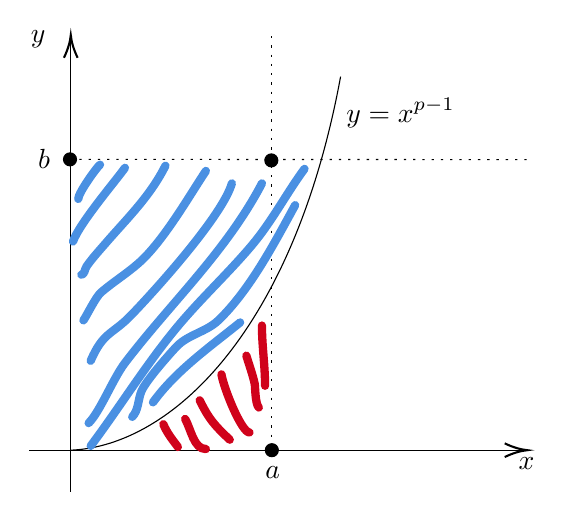
\begin{tikzpicture}[x=0.75pt,y=0.75pt,yscale=-1,xscale=1]
%uncomment if require: \path (0,300); %set diagram left start at 0, and has height of 300

%Straight Lines [id:da6670187171435178] 
\draw    (20,270) -- (258,270) ;
\draw [shift={(260,270)}, rotate = 180] [color={rgb, 255:red, 0; green, 0; blue, 0 }  ][line width=0.75]    (10.93,-3.29) .. controls (6.95,-1.4) and (3.31,-0.3) .. (0,0) .. controls (3.31,0.3) and (6.95,1.4) .. (10.93,3.29)   ;
%Straight Lines [id:da5739587577361009] 
\draw    (40,290) -- (40,72) ;
\draw [shift={(40,70)}, rotate = 450] [color={rgb, 255:red, 0; green, 0; blue, 0 }  ][line width=0.75]    (10.93,-3.29) .. controls (6.95,-1.4) and (3.31,-0.3) .. (0,0) .. controls (3.31,0.3) and (6.95,1.4) .. (10.93,3.29)   ;
%Curve Lines [id:da9000590437864551] 
\draw    (40,270) .. controls (89.1,267.95) and (147.6,211.45) .. (170,90) ;
%Flowchart: Connector [id:dp45258608048860904] 
\draw  [fill={rgb, 255:red, 0; green, 0; blue, 0 }  ,fill opacity=1 ] (133.75,270) .. controls (133.75,268.27) and (135.15,266.88) .. (136.88,266.88) .. controls (138.6,266.88) and (140,268.27) .. (140,270) .. controls (140,271.73) and (138.6,273.13) .. (136.88,273.13) .. controls (135.15,273.13) and (133.75,271.73) .. (133.75,270) -- cycle ;
%Flowchart: Connector [id:dp8047377936424447] 
\draw  [fill={rgb, 255:red, 0; green, 0; blue, 0 }  ,fill opacity=1 ] (36.5,129.88) .. controls (36.5,128.15) and (37.9,126.75) .. (39.63,126.75) .. controls (41.35,126.75) and (42.75,128.15) .. (42.75,129.88) .. controls (42.75,131.6) and (41.35,133) .. (39.63,133) .. controls (37.9,133) and (36.5,131.6) .. (36.5,129.88) -- cycle ;
%Straight Lines [id:da4410313174304634] 
\draw  [dash pattern={on 0.84pt off 2.51pt}]  (39.63,129.88) -- (260,130) ;
%Straight Lines [id:da5523219504500843] 
\draw  [dash pattern={on 0.84pt off 2.51pt}]  (136.88,70.45) -- (136.88,270) ;
%Flowchart: Connector [id:dp41859750439357146] 
\draw  [fill={rgb, 255:red, 0; green, 0; blue, 0 }  ,fill opacity=1 ] (133.5,130.38) .. controls (133.5,128.65) and (134.9,127.25) .. (136.63,127.25) .. controls (138.35,127.25) and (139.75,128.65) .. (139.75,130.38) .. controls (139.75,132.1) and (138.35,133.5) .. (136.63,133.5) .. controls (134.9,133.5) and (133.5,132.1) .. (133.5,130.38) -- cycle ;
%Shape: Free Drawing [id:dp7605874538730915] 
\draw  [color={rgb, 255:red, 74; green, 144; blue, 226 }  ,draw opacity=1 ][line width=3] [line join = round][line cap = round] (54.1,132.45) .. controls (52.77,133.34) and (43.6,146.01) .. (43.6,148.95) ;
%Shape: Free Drawing [id:dp8118651084447608] 
\draw  [color={rgb, 255:red, 74; green, 144; blue, 226 }  ,draw opacity=1 ][line width=3] [line join = round][line cap = round] (66.1,133.95) .. controls (62.38,139.33) and (43.97,160.85) .. (41.1,169.45) ;
%Shape: Free Drawing [id:dp47624921947753585] 
\draw  [color={rgb, 255:red, 74; green, 144; blue, 226 }  ,draw opacity=1 ][line width=3] [line join = round][line cap = round] (85.6,132.95) .. controls (78.3,147.55) and (67.47,157.98) .. (57.1,169.95) .. controls (53.84,173.71) and (50.45,177.38) .. (47.6,181.45) .. controls (46.7,182.74) and (46.67,185.45) .. (45.1,185.45) ;
%Shape: Free Drawing [id:dp1350010769424319] 
\draw  [color={rgb, 255:red, 74; green, 144; blue, 226 }  ,draw opacity=1 ][line width=3] [line join = round][line cap = round] (105.1,135.45) .. controls (97.14,147.38) and (84.56,169.46) .. (72.6,179.95) .. controls (66.89,184.96) and (60.38,189.01) .. (54.6,193.95) .. controls (52.04,196.13) and (47.74,205.07) .. (46.1,207.45) ;
%Shape: Free Drawing [id:dp7004032676837966] 
\draw  [color={rgb, 255:red, 74; green, 144; blue, 226 }  ,draw opacity=1 ][line width=3] [line join = round][line cap = round] (117.6,141.45) .. controls (113.24,156.72) and (81.89,191.65) .. (69.1,204.95) .. controls (60.04,214.37) and (55.64,212.86) .. (49.6,226.95) ;
%Shape: Free Drawing [id:dp31434135159409937] 
\draw  [color={rgb, 255:red, 74; green, 144; blue, 226 }  ,draw opacity=1 ][line width=3] [line join = round][line cap = round] (132.1,141.45) .. controls (115.02,174.18) and (88.09,199.09) .. (66.1,227.95) .. controls (60.34,235.5) and (54.17,251.38) .. (48.6,256.95) ;
%Shape: Free Drawing [id:dp6894175047204754] 
\draw  [color={rgb, 255:red, 74; green, 144; blue, 226 }  ,draw opacity=1 ][line width=3] [line join = round][line cap = round] (152.6,134.45) .. controls (143.7,146.58) and (136.85,159.92) .. (127.1,171.45) .. controls (115.54,185.12) and (102.04,197.56) .. (90.6,211.45) .. controls (75.82,229.4) and (63.08,249.97) .. (49.6,267.95) ;
%Shape: Free Drawing [id:dp8278177576754198] 
\draw  [color={rgb, 255:red, 74; green, 144; blue, 226 }  ,draw opacity=1 ][line width=3] [line join = round][line cap = round] (148.1,151.95) .. controls (138.2,170.01) and (126.36,192.8) .. (111.1,207.45) .. controls (105.32,212.99) and (96.63,214.26) .. (91.1,219.95) .. controls (89.27,221.83) and (76.47,235.97) .. (74.1,241.45) .. controls (72.34,245.51) and (72.73,250.82) .. (69.6,253.95) ;
%Shape: Free Drawing [id:dp8368556323111096] 
\draw  [color={rgb, 255:red, 74; green, 144; blue, 226 }  ,draw opacity=1 ][line width=3] [line join = round][line cap = round] (121.6,208.45) .. controls (106.91,220.34) and (90.76,231.6) .. (79.6,246.95) ;
%Shape: Free Drawing [id:dp568158357605342] 
\draw  [color={rgb, 255:red, 208; green, 2; blue, 27 }  ,draw opacity=1 ][line width=3] [line join = round][line cap = round] (84.6,257.45) .. controls (86.23,261.51) and (88.9,264.85) .. (91.6,268.45) ;
%Shape: Free Drawing [id:dp1743471495118334] 
\draw  [color={rgb, 255:red, 208; green, 2; blue, 27 }  ,draw opacity=1 ][line width=3] [line join = round][line cap = round] (95.1,254.95) .. controls (98.01,260.05) and (99.23,269.45) .. (105.1,269.45) ;
%Shape: Free Drawing [id:dp7057820022191483] 
\draw  [color={rgb, 255:red, 208; green, 2; blue, 27 }  ,draw opacity=1 ][line width=3] [line join = round][line cap = round] (102.1,245.95) .. controls (106.57,254.89) and (108.76,257.55) .. (116.6,264.95) ;
%Shape: Free Drawing [id:dp3036581460753516] 
\draw  [color={rgb, 255:red, 208; green, 2; blue, 27 }  ,draw opacity=1 ][line width=3] [line join = round][line cap = round] (112.6,233.45) .. controls (113.77,240.44) and (122.29,261.45) .. (126.1,261.45) ;
%Shape: Free Drawing [id:dp11642496827327031] 
\draw  [color={rgb, 255:red, 208; green, 2; blue, 27 }  ,draw opacity=1 ][line width=3] [line join = round][line cap = round] (124.6,224.45) .. controls (125.93,228.95) and (127.59,233.37) .. (128.6,237.95) .. controls (128.89,239.26) and (128.79,247.64) .. (130.6,249.45) ;
%Shape: Free Drawing [id:dp2760707325831322] 
\draw  [color={rgb, 255:red, 208; green, 2; blue, 27 }  ,draw opacity=1 ][line width=3] [line join = round][line cap = round] (132.1,209.95) .. controls (132.1,219.68) and (133.6,229.22) .. (133.6,238.95) ;

% Text Node
\draw (132.5,276.7) node [anchor=north west][inner sep=0.75pt]   [align=left] {$\displaystyle a$};
% Text Node
\draw (23,123.7) node [anchor=north west][inner sep=0.75pt]   [align=left] {$\displaystyle b$};
% Text Node
\draw (254.5,272.2) node [anchor=north west][inner sep=0.75pt]   [align=left] {$\displaystyle x$};
% Text Node
\draw (19.5,66.7) node [anchor=north west][inner sep=0.75pt]   [align=left] {$\displaystyle y$};
% Text Node
\draw (171.5,99.2) node [anchor=north west][inner sep=0.75pt]   [align=left] {$\displaystyle y=x^{p-1}$};


\end{tikzpicture}

        \end{center}
    \end{remark}
\end{theorem}

\begin{theorem}[неравенство Минковского]
    Если $f,\, g\in L^p$, $p\in[1,\, +\infty]$, то \[
        \|f+g\|_p\leqslant\|f\|_p+\|g\|_p.
    \]
\end{theorem}
